\chapter{Language models}


\section{Spelling correction}

\begin{description}
    \item[Spelling correction] \marginnote{Spelling correction}
        Spelling errors can be of two types:
        \begin{description}
            \item[Non-word spelling] 
                Typos that result in non-existing words. Possible candidates can be determined though a dictionary lookup.
        
            \item[Real-word spelling] 
                Can be:
                \begin{description}
                    \item[Typographical error] Typos that result in existing words.
                    \item[Cognitive error] Due to words similarity (e.g., \texttt{piece} vs \texttt{peace}).
                \end{description}
        \end{description}
\end{description}

% \textbf{Rank a list of candidates based on a distance metric (e.g., minimum edit distance). Also consider word frequency and likelihood in the context.}


\begin{description}
    \item[Noisy channel model] \marginnote{Noisy channel model}
        Assumes that the observable input is a distorted form of the original word. A decoder tests word hypotheses and selects the best match. 

        \begin{minipage}{0.7\linewidth}
            More formally, we want a model of the channel that, similarly to Bayesian inference, determines the likelihood that a word $w \in V$ is the original word for a noisy one $x$. From there, we can estimate the correct word $\hat{w}$:
            \[ \hat{w} = \arg\max_{w \in V} \prob{w | x} \]
            By applying 
            \begin{enumerate*}[label=(\roman*)]
                \item Bayes' rule, 
                \item the fact that $\hat{w}$ is independent of $\prob{x}$, and
                \item that a subset $C \subseteq V$ of the vocabulary can be used,
              \end{enumerate*}
            the estimate becomes:
            \[ \hat{w} = \arg\max_{w \in C} \underbrace{\prob{x|w}}_{\text{channel model}} \underbrace{\prob{w}}_{\text{prior}} \]

            Moreover, it is reasonable to include a context $c$ when computing the prior:
            \[ \hat{w} = \arg\max_{w \in C} \underbrace{\prob{x|w}}_{\text{channel model}} \underbrace{\prob{w|c}}_{\text{ language model}} \]
        \end{minipage}
        \hfill
        \begin{minipage}{0.27\linewidth}
            \begin{figure}[H]
                \centering
                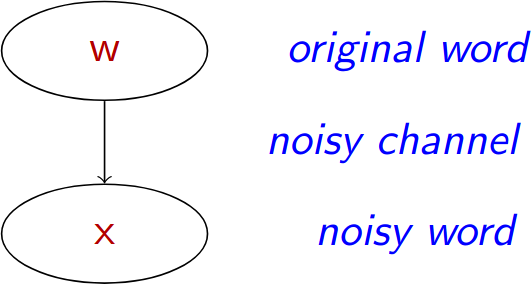
\includegraphics[width=\linewidth]{./img/noisy_channel1.png}
            \end{figure}
            \vspace{2.5em}
            \begin{figure}[H]
                \centering
                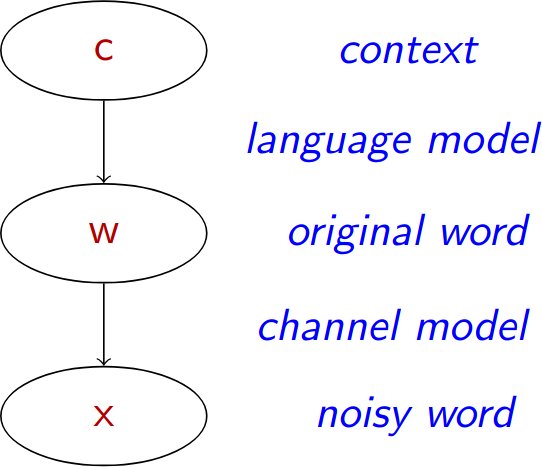
\includegraphics[width=\linewidth]{./img/noisy_channel2.png}
            \end{figure}
        \end{minipage}

    \item[Noisy channel spelling method]
        Spelling correction in a noisy channel model can be done as follows:
        \begin{enumerate}
            \item Find candidate words with similar spelling to the input based on a distance metric (e.g., Damerau-Levenshtein which is the Levenshtein distance with the addition of adjacent transpositions).
            \item Score each candidate based on the language and channel model:
            \begin{itemize}
                \item Use typing features of the user.
                \item Use local context.
                \item Use a confusion matrix with common mistakes.
            \end{itemize}
        \end{enumerate}
\end{description}

\begin{example}
    Consider the sentence:
    \begin{center}
        \parbox{0.65\linewidth}{
            \textit{\textnormal{[...]} was called a ``stellar and versatile \texttt{acress} whose combination of sass and glamour has defined her \textnormal{[...]}''}
        }
    \end{center}
    By using the Corpus of Contemporary American English (COCA), we can determine the following words as candidates:
    \[
        \texttt{actress} \cdot \texttt{cress} \cdot \texttt{caress} \cdot \texttt{access} \cdot \texttt{across} \cdot \texttt{acres}
    \]

    \begin{description}
        \item[Language model] By considering a language model without context, the priors are computed as $\prob{w | \varepsilon} = \frac{\texttt{count}(w)}{\vert \texttt{COCA} \vert}$ (where $\vert \texttt{COCA} \vert = \num{404253213}$):
        \begin{table}[H]
            \centering
            \footnotesize
            \begin{tabular}{ccl}
                \toprule
                $w$ & $\texttt{count}(w)$ & $\prob{w | \varepsilon}$ \\
                \midrule
                \texttt{actress}    & \num{9321}    & $0.0000231$   \\
                \texttt{cress}      & \num{220}     & $0.000000544$ \\
                \texttt{caress}     & \num{686}     & $0.00000170$  \\
                \texttt{access}     & \num{37038}   & $0.0000916$   \\
                \texttt{across}     & \num{120844}  & $0.000299$    \\
                \texttt{acres}      & \num{12874}   & $0.0000318$   \\
                \bottomrule
            \end{tabular}
        \end{table}

        \item[Channel model] 
            By using a confusion matrix of common typos, the channel model is:
            \begin{table}[H]
                \centering
                \footnotesize
                \begin{tabular}{ccl}
                    \toprule
                    $w$ & $x | w$ & $\prob{x | w}$ \\
                    \midrule
                    \texttt{actress} & $\texttt{c}|\texttt{ct}$  & $0.000117$ \\
                    \texttt{cress}   & $\texttt{a}|\texttt{\#}$  & $0.00000144$ \\
                    \texttt{caress}  & $\texttt{ac}|\texttt{ca}$ & $0.00000164$ \\
                    \texttt{access}  & $\texttt{r}|\texttt{c}$   & $0.000000209$ \\
                    \texttt{across}  & $\texttt{e}|\texttt{o}$   & $0.0000093$ \\
                    \texttt{acres}   & $\texttt{es}|\texttt{e}$  & $0.0000321$ \\
                    \texttt{acres}   & $\texttt{ss}|\texttt{s}$  & $0.0000342$ \\
                    \bottomrule
                \end{tabular}
            \end{table}
    \end{description}

    The ranking is the obtained as:
    \begin{table}[H]
        \centering
        \footnotesize
        \begin{tabular}{cl}
            \toprule
            $w$ & $\prob{x | w} \prob{w | \varepsilon}$ \\
            \midrule
            \texttt{actress} & $2.7 \cdot 10^{-9}$ \\
            \texttt{cress}   & $0.00078 \cdot 10^{-9}$ \\
            \texttt{caress}  & $0.0028 \cdot 10^{-9}$ \\
            \texttt{access}  & $0.019 \cdot 10^{-9}$ \\
            \texttt{across}  & $2.8 \cdot 10^{-9}$ \\
            \texttt{acres}   & $1.02 \cdot 10^{-9}$ \\
            \texttt{acres}   & $1.09 \cdot 10^{-9}$ \\
            \bottomrule
        \end{tabular}
    \end{table}

    Therefore, the most likely correction of \texttt{acress} for this model is \texttt{across}.

    If the previous word is considered in the context, the relevant tokens of the new language model are:
    \begin{table}[H]
        \centering
        \footnotesize
        \begin{tabular}{ccl}
            \toprule
            $w_{i-1}$ & $w_i$ & $\prob{w_i | w_{i-1}}$ \\
            \midrule
            \texttt{versatile} & \texttt{actress}   & $0.000021$ \\
            \texttt{versatile} & \texttt{across}    & $0.000021$ \\
            \texttt{actress}   & \texttt{whose}     & $0.001$ \\
            \texttt{across}    & \texttt{whose}     & $0.000006$ \\
            \bottomrule
        \end{tabular}
    \end{table}
    This allows to measure the likelihood of a sentence as:
    \[
        \begin{split}
            \prob{\texttt{versatile \underline{actress} whose}} &= \prob{\texttt{actress} | \texttt{versatile}} \prob{\texttt{whose} | \texttt{actress}} = 210 \cdot 10^{-10} \\
            \prob{\texttt{versatile \underline{across} whose}} &= \prob{\texttt{across} | \texttt{versatile}} \prob{\texttt{whose} | \texttt{across}} = 1 \cdot 10^{-10}
        \end{split}
    \]
    Finally, we have that:
    \[
        \begin{split}
            \prob{\texttt{versatile \underline{actress} whose} | \texttt{versatile acress whose}} &= (2.7 \cdot 10^{-9}) \cdot (210 \cdot 10^{-10}) \\
            \prob{\texttt{versatile \underline{across} whose} | \texttt{versatile acress whose}} &= (2.8 \cdot 10^{-9}) \cdot (1 \cdot 10^{-10}) \\
        \end{split}
    \]
    So \texttt{actress} is the most likely correction for \texttt{acress} in this model.
\end{example}


\begin{remark}
    In practice, log-probabilities are used to avoid underflows and to make computation faster (i.e., sums instead of products).
\end{remark}



\section{Language models}

\begin{description}
    \item[(Probabilistic) language model] \marginnote{Language model}
        Model to determine the probability of a word $w$ in a given context $c$:
        \[ \prob{w | c} \]
        Usually, it is based on counting statistics and uses as context the sequence of previous tokens:
        \[ \prob{w_i | w_1, \dots, w_{i-1}} \]
        This is equivalent to computing the probability of the whole sentence, which expanded using the chain rule becomes:
        \[
            \begin{split}
                \prob{w_1, \dots, w_{i-1} w_i} &= \prob{w_1} \prob{w_2 | w_1} \prob{w_3 | w_{1..2}} \dots \prob{w_n | w_{1..n-1}} \\
                &= \prod_{i=1}^{n} \prob{w_i | w_{1..i-1}}
            \end{split}
        \]

        \begin{remark}
            Simply counting the number of occurrences of a sentence as $\prob{w_i | w_{1..i-1}} = w_{1..i} / w_{1..i-1}$ is not ideal as there are too many possible sentences.
        \end{remark}

    \item[Markov assumption] \marginnote{Markov assumption in language models}
        Limit the length of the context to a window of $k$ previous tokens:
        \[ \prob{w_i | w_{1..i-1}} \approx \prob{w_i | w_{i-k..i-1}} \]
        \[ \prob{w_{1..n}} \approx \prod_{i=1}^{n} \prob{w_i | w_{i-k..i-1}} \]

        \begin{description}
            \item[Unigram model]
                Model without context ($k=0$):
                \[ \prob{w_{1..n}} \approx \prod_i \prob{w_i} \]

            \item[Bigram model]
                Model with a single token context ($k=1$):
                \[ \prob{w_{1..n}} \approx \prod_i \prob{w_i | w_{i-1}} \]

            \item[$\mathbf{N}$-gram model] \marginnote{$N$-gram model}
                Model with a context of $k=N-1$ tokens:
                \[ \prob{w_{1..n}} \approx \prod_i \prob{w_i | w_{i-N+1..i-1}} \]

                \begin{remark}
                    $N$-gram models cannot capture long-range dependencies.
                \end{remark}

                \begin{description}
                    \item[Estimating $\mathbf{N}$-gram probabilities]
                        Consider the bigram case, the probability that a token $w_i$ follows $w_{i-1}$ can be determined through counting:
                        \[ \prob{w_i | w_{i-1}} = \frac{\texttt{count}(w_{i-1} w_i)}{\texttt{count}(w_{i-1})} \]
                \end{description}

                \begin{remark}
                    $N$-gram models cannot handle unknown tokens.
                \end{remark}

                \begin{remark}
                    $N$-gram models capture knowledge about:
                    \begin{itemize}
                        \item Grammar and syntax.
                        \item Some information about the dataset (e.g., domain, genre of corpus, cultural aspects, \dots).
                    \end{itemize}
                \end{remark}
        \end{description}

    \item[Generation by sampling] \marginnote{Generation by sampling}
        Randomly sample tokens from the distribution of a language model.

        \begin{remark}
            In $N$-gram models ($N \geq 2$), the distribution changes depending on the previously sampled tokens.
        \end{remark}
\end{description}



\section{Metrics}


\subsection{Extrinsic evaluation}

\begin{description}
    \item[Extrinsic/downstream evaluation] \marginnote{Extrinsic evaluation}
        Compare the performance of different models on specific tasks.
\end{description}

\begin{remark}
    Extrinsic evaluation is the best approach for comparing different models, but it is often computationally expensive.
\end{remark}


\subsection{Intrinsic evaluation}

\begin{description}
    \item[Intrinsic evaluation] \marginnote{Intrinsic evaluation}
        Measure the quality of a model independently of the task.

    \item[Perplexity (\texttt{PP})] \marginnote{Perplexity}
        Probability-based metric based on the inverse probability of a sequence (usually using the test set) normalized by the number of words:
        \[
            \begin{split}
                \prob{w_{1..N}} &= \prod_{i} \prob{w_i | w_{1..i-1}} \\
                \texttt{PP}(w_{1..N}) &= \prob{w_{1..N}}^{-\frac{1}{N}} \in [1, +\infty]
            \end{split}
        \]
        Generally, a lower perplexity represents a better model.

        \begin{example}
            For bigram models, perplexity is computed as:
            \[ 
                \prob{w_{1..N}} \approx \prod_{i} \prob{w_i | w_{i-1}}
                \qquad
                \texttt{PP}(w_{1..N}) = \sqrt[N]{\prod_{i} \frac{1}{\prob{w_i | w_{i-1}}}}
            \]
        \end{example}

        \begin{remark}[Perplexity intuition]
            Perplexity can be seen as a measure of surprise of a language model when evaluating a sequence.

            Alternatively, it can also be seen as a weighted average branching factor (i.e., average number of possible unique next words that follow any word, accounting for their probabilities). For instance, consider a vocabulary of digits and a training corpus where every digit appears with uniform probability $0.1$. The perplexity of any sequence using a 1-gram model is:
            \[ \texttt{PP}(w_{1..N}) = \left( 0.1^{N} \right)^{-\frac{1}{N}} = 10 \]
            Now consider a training corpus where $0$ occurs $91\%$ of the time and the other digits $1\%$ of the time. The perplexity of the sequence \texttt{0 0 0 0 0 3 0 0 0 0} is:
            \[ \texttt{PP}(\texttt{0 0 0 0 0 3 0 0 0 0}) = \left( 0.91^9 \cdot 0.01 \right)^{-\frac{1}{10}} \approx 1.73 \]
        \end{remark}

        \begin{remark}
            Minimizing perplexity is the same as maximizing the probability of the tokens.
        \end{remark}

        \begin{remark}
            Perplexity can be artificially reduced by using a smaller vocabulary. Therefore, it is only reasonable to compare perplexity of models with the same vocabulary.
        \end{remark}

        \begin{remark}
            Perplexity is generally a bad approximation of extrinsic metrics and only works well if the test set is representative of the training data. Therefore, it is only useful to guide experiments and the final evaluation should be done through extrinsic evaluation.
        \end{remark}
\end{description}



\section{$\mathbf{N}$-gram model problems}


\subsection{Overfitting}
\marginnote{Overfitting}

$N$-gram models become better at modeling the training corpus for increasing values of $N$. This risks overfitting and does not allow to obtain a generalized model.

\begin{example}
    A 4-gram model is able to nearly perfectly generate sentences from Shakespeare's works.
\end{example}


\subsection{Out-of-vocabulary tokens}

There are two types of vocabulary systems:
\begin{descriptionlist}
    \item[Closed vocabulary system] \marginnote{Closed vocabulary}
        All words that can occur are known.

    \item[Open vocabulary system] \marginnote{Open vocabulary}
        Unknown words are possible. They are usually handled using a dedicated token \texttt{<UNK>} which allows to turn an open vocabulary system into a closed one:
        \begin{itemize}
            \item Use a vocabulary and model all other words as \texttt{<UNK>}.
            \item Model infrequent words as \texttt{<UNK>}.
        \end{itemize}

        \begin{remark}
            The training set must contain \texttt{<UNK>} tokens to estimate its distribution as it is treated as any other token.
        \end{remark}
\end{descriptionlist}


\subsection{Unseen sequences}

Only for $n$-grams that occur enough times a representative probability can be estimated. For increasing values of $n$, the sparsity grows causing many unseen $n$-grams that produce a probability of $0$, with the risk of performing divisions by zero (e.g., when computing perplexity) or zeroing probabilities (e.g., when applying the chain rule).

\begin{description}
    \item[Laplace smoothing] \marginnote{Laplace smoothing}
        Adds $1$ to all counts and renormalizes them. Given a vocabulary $V$ and an $N$-gram model, smoothing is done as follows:
        \[
            \mathcal{P}_\text{Laplace}(w_i | w_{i-N+1..i-1}) = \frac{\texttt{count}(w_{i-N+1..i-1}w_i) + 1}{\texttt{count}(w_{i-N+1..i-1}) + \vert V \vert}
        \]
        Alternatively, by only changing the numerator, it can be formulated using an adjusted count as:
        \[
            \begin{gathered}
                \mathcal{P}_\text{Laplace}(w_i | w_{i-N+1..i-1}) = \frac{c^*}{\texttt{count}(w_{i-N+1..i-1})} \\
                c^* = \big( \texttt{count}(w_{i-N+1..i-1}w_i) + 1 \big) \frac{\texttt{count}(w_{i-N+1..i-1})}{\texttt{count}(w_{i-N+1..i-1}) + \vert V \vert}
            \end{gathered}
        \]
        where $\frac{\texttt{count}(w_{i-N+1..i-1})}{\texttt{count}(w_{i-N+1..i-1}) + \vert V \vert}$ is a normalization factor.

        \begin{example}
            For a 2-gram model, Laplace smoothing is computed as:
            \[
                \mathcal{P}_\text{Laplace}(w_i | w_{i-1}) = \frac{\texttt{count}(w_{i-1}w_i) + 1}{\texttt{count}(w_{i-1}) + \vert V \vert}
            \]
            Or by using the adjusted count as:
            \[
                \mathcal{P}_\text{Laplace}(w_i | w_{i-1}) = \frac{c^*}{\texttt{count}(w_{i-1})}
                \qquad
                c^* = \big( \texttt{count}(w_{i-1}w_i) + 1 \big) \frac{\texttt{count}(w_{i-1})}{\texttt{count}(w_{i-1}) + \vert V \vert}
            \]
        \end{example}
\end{description}